\chapter{Enabling Structured Illumination Microscopy at greater depth}

\section{Sample Induced Aberrations in Thick Samples}
\label{sec:sample_aberrations_thick}

\begin{itemize}
	\item Recap sample induced aberrations and how they impair SIM imaging in-particular
\end{itemize}

\subsection{Scattering Aberrations}
\label{subsec:scattering}

\begin{itemize}
	\item Worth highlighting that at a certain point, you lose image quality to scattering aberrations which AO can't help with.
\end{itemize}

\section{Sensorless Adaptive Optics}
\label{sec:sensorless_AO}

\subsection{Image Quality Metric: Fourier Power}
\label{subsec:fourier_power_metric}

As mentioned in Section~\ref{subsubsec:sensorless_correction}, 
sensorless AO correction requires an image quality metric which
is well suited to both the imaging modality and the desired 
sample. Microscope-AOtools implements a suite of image quality
metrics to choose from. Since SIM data is contingent on high
quality Fourier information, a sensible starting point for 
the image quality metric, $S$, is the total power of the Fourier
spectrum:

\begin{equation}\label{eq:fourier_power_spectrum}
S = \sum\limits_{n,m}{\vline \tilde{\textbf{D}}_{n,m} \vline^2}
\end{equation}

Where $\tilde{\textbf{D}}$ is the 2D discrete Fourier transform of 
the observed fluorescent signal and $n$ and $m$ are the pixel coordinates 
with ranges $[0, N-1]$ and $[0, M-1]$ respectively, where $N$ and $M$ are the
number of pixels along each dimension of the image. From Parseval's Theorem, 
$\sum\limits_{n,m}\vline \tilde{\textbf{D}}_{n,m} \vline^2$ is
the power of the observed signal. However, the Fourier spectrum
obtained is not entirely composed of sample information. The 
fluorescent signal is the convolution of the distribution of fluorescent 
emission, $E(\bar{r})$, and the system point spread function (PSF), 
$H(\bar{r})$: 

\begin{equation}\label{eq:fluor_signal_real}
D(\bar{r}) = (E \circledast H)(\bar{r})
\end{equation}

In Fourier space, this convolution becomes $\tilde{\textbf{D}}(\bar{k}) 
= \tilde{\textbf{E}}(\bar{k}) \tilde{\textbf{H}}(\bar{k}) = 
\tilde{\textbf{E}}(\bar{k}) \textbf{O}(\bar{k})$, where the tilde ($\sim$)
represent the Fourier transform of the corresponding real-space functions and 
$\textbf{O}(\bar{k})$ is the system optical transfer function (OTF).\cite{gustafsson2008three} The OTF both attenuates the sample structure spatial frequencies and acts as
a lowpass filter. Since $\tilde{\textbf{D}}_{n,m}$ is the 2D discrete
Fourier transform of the observed data, this lowpass filter, $\mu_{n,m}$, is
defined as:

\begin{equation}\label{eq:circular_mask}
\mu_{n,m} = 
\begin{cases}
1, & \sqrt{n'^{2} + m'^{2}} \le w\\
0, & \sqrt{n'^{2} + m'^{2}} > w\\ 
\end{cases}
\end{equation}

Where $n' = n - \frac{N-1}{2}$, $m' = m - \frac{M-1}{2}$ and $w$ a radius 
defined as the size of the field of view of the image divided by the Abbe
diffraction limit for the system, $\frac{1.22\lambda}{2NA}$.\cite{abbe1873beitrage} 

Within the OTF lowpass limit, certain spatial frequencies will be dominated
by noise contributions. As such, when attempting to quantify the power 
contribution from the fluorescent it is desirable to ignore the noise
contributions. A thresholding mask, $\tau_{n,m}$ is created and defined as:

\begin{equation}\label{eq:noise_threshold_mask}
\tau_{n,m} = 
\begin{cases}
0, & \vline \tilde{\textbf{D}}_{n,m} \vline^2 < \delta\\
1, & \vline \tilde{\textbf{D}}_{n,m} \vline^2 \ge \delta\\ 
\end{cases}
\end{equation}

Where $\delta$ is a noise threshold defined as:

\begin{equation}\label{eq:noise_threshold}
\delta = \frac{\alpha}{P_{noise}}\sum\limits_{l,k}{\vline \tilde{\textbf{D}}_{l,k} \vline^2}
\end{equation}

Where $\vline \tilde{\textbf{D}}_{l,k} \vline^2$ is the power in the 
$l$-th, $k$-th spatial frequency where $l$ \& $k$ are the coordinates 
where $\mu_{n,m} = 0$, $P_{noise}$ is the total number of pixels 
outside the OTF lowpass limit and $\alpha$ is a user defined 
amplification factor. In essence, the threshold is the mean of the
power of the spatial frequencies consisting entirely of noise signals,
scaled by $\alpha$.	The value of $\alpha$ must be chosen to threshold
the spatial frequencies dominated by noise without losing the sensitivity
to true, albeit low amplitude, spatial frequencies. Empirically, an 
$\alpha = 1.125$ offers a reasonable compromise between these traits.

Finally, the bulk of the improvement in spatial frequency content will
occur in the mid to high frequencies (relative to $w$). As such there is 
a desire for increased sensitivity to the power fluctuations in these 
spatial frequencies. A modulation mask, $\omega$, is constructed and 
defined as:

\begin{equation}\label{eq:attenuation_mask_norm_and_scaled}
\omega_{n,m} = \beta \vline (1 - e^{\frac{\sqrt{n'^{2} + m'^{2}}}{w}-1}) (n'^{2} + m'^{2}) \vline
\end{equation}

Where $w$, $n'$ and $m'$ are defined as before, $\vline\textbf{x} \vline$ 
is $\textbf{x}$ normalised to $[0,1]$, and $\beta$ is a user defined 
normalisation factor. In effect, this modulation mask amplifies the mid 
to high spatial frequencies while attenuating the low spatial frequencies 
and the high spatial frequency noise close to $w$.

Applying these modification to Equation~\ref{eq:fourier_power_spectrum} 
yields the image quality metric:

\begin{equation}\label{eq:Fourier_power_metric}
S = \sum\limits_{n,m}{\mu_{n,m}\tau_{n,m}\omega_{n,m}\vline \tilde{\textbf{D}}_{n,m} \vline^2}
\end{equation}

Where $\mu_{n,m}$, $\tau_{n,m}$ and $\omega_{n,m}$ are defined as in
Equations~\ref{eq:circular_mask},~\ref{eq:noise_threshold_mask} and
\ref{eq:attenuation_mask_norm_and_scaled} respectively and 
$\tilde{\textbf{D}}_{n,m}$ is defined as before. In practice, $S$
measures the total power of the sample spatial frequencies, with 
increased sensitivity to mid to high spatial frequency changes. As
such, this image quality metric is called the Fourier Power metric.
Since SIM imaging depends on high quality spatial frequency 
information, this image quality metric is particularly well suited 
to correcting aberrations for SIM data.

\subsection{IsoSense}
\label{subsec:isosense}

Anisotropies in the sample structure can bias the corrections
towards improving the image quality in a non-uniform manner.
There has recently been a technique developed to overcome 
this issue; IsoSense\cite{vzurauskas2019isosense}. It relies 
on producing spatially structured light in order to fill 
empty sections of the image Fourier spectrum. IsoSense is 
designed to be used in structured illumination microscopy 
(SIM) setups since they often incorporate spatial light 
modulators (SLM) as high-speed, dynamic diffraction 
gratings and SIM is particularly sensitive to Fourier
space anisotropies.

Microscope-AOtools incorporates the methods necessary to implement
IsoSense. Figure~\ref{fig:isosense_visualisation} shows both
the structured illumination pattern applied to the SLM 
and the location of the beams in Fourier space. The illumination
pattern shown in Figure~\ref{fig:isosense_visualisation_real} is
the inverse Fourier transform of the 4-beam interference pattern 
in Figure~\ref{fig:isosense_visualisation_ft}. The location 
of these beams, $\bar{\kappa}$, are: 
$(0,0)$, $(0,\gamma w)$, $(0,-\gamma w)$, $(\gamma w, 0)$, 
$(-\gamma w, 0)$, $(\frac{\gamma w}{2}, \frac{\gamma w}{2})$, 
$(-\frac{\gamma w}{2}, \frac{\gamma w}{2})$, $(\frac{\gamma w}{2},
-\frac{\gamma w}{2})$, $(-\frac{\gamma w}{2}, 
-\frac{\gamma w}{2})$. $u,v$ are the spatial frequency 
analogues of the $x,y$ axes. $w$ is the Abbe diffraction limit and 
$\gamma$ is a user defined fill fraction. This fill
fraction controls the positions of the beams in the interference
pattern and hence the region of the Fourier spectrum which will 
be enhanced over normal illumination. The resultant fluorescent image 
obtained, $F(x,y)$, can be described as:

\begin{equation}\label{eq:isosense_real}
F(\bar{r}) = D(\bar{r}) \times I(\bar{r})
\end{equation}	

Where $I(\bar{r})$ is the interference pattern, similar to that shown in 
Figure\ref{fig:isosense_visualisation_real} and $E(\bar{r})$ is the sample
structure as before. Applying a Fourier transform yields:

\begin{equation}\label{eq:isosense_ft}
\begin{split}
\mathcal{F}[F(\bar{r})] &= \mathcal{F}[D(\bar{r})\times I(\bar{r})] \\
\tilde{\textbf{F}}(\bar{k}) &= \tilde{\textbf{D}}(\bar{k}) \circledast \tilde{\textbf{I}}(\bar{k}) \\
\tilde{\textbf{F}}(\bar{k}) &= \sum_{\bar{\kappa}}\iint\tilde{\textbf{D}}(\bar{k})\delta(\bar{k} - \bar{\kappa})dudv \\
\tilde{\textbf{F}}(\bar{k}) &= \sum_{\bar{\kappa}}\tilde{\textbf{D}}(\bar{k} - \bar{\kappa})
\end{split}
\end{equation}

Where $\tilde{\textbf{F}}(\bar{k})$, $\tilde{\textbf{I}}(\bar{k})$ and 
$\tilde{\textbf{D}}(\bar{k})$ are the Fourier transforms of $F(\bar{r})$, 
$I(\bar{r})$ and $D(\bar{r})$, the $\bar{\kappa}$ frequencies are the 
locations of interference pattern beams described above. By convolving 
the sample structure with multiple $\delta$-functions, multiple copies 
of the sample spatial frequency information are created and regions of 
the system OTF left unfilled by sample structure anisotropies are 
filled, leading to improved sampling of the system OTF particularly
at high spatial frequencies close to $w$ and greater aberration
sensitivity.\cite{vzurauskas2019isosense}

\begin{figure}[h]
	\centering
	\begin{subfigure}{0.4\textwidth}
		\centering
		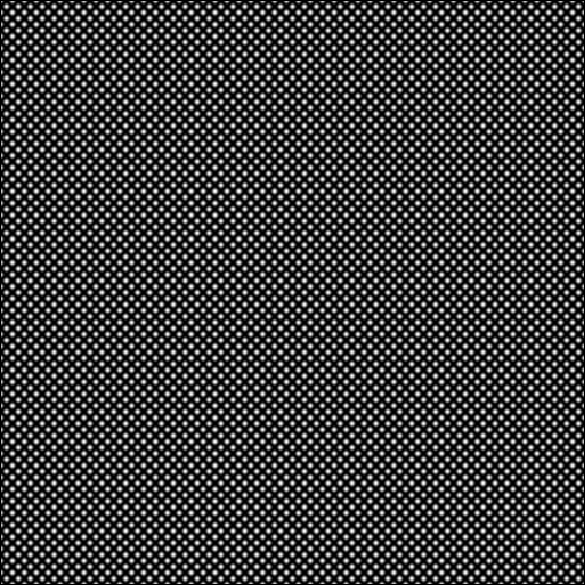
\includegraphics[width=1\linewidth, scale=0.5]{./images/isosense_visualisation_real.png}
		\caption{}
		\label{fig:isosense_visualisation_real}
	\end{subfigure}
	\begin{subfigure}{0.4\textwidth}
		\centering
		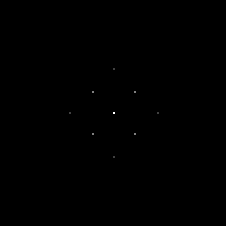
\includegraphics[width=1\linewidth, scale=0.5]{./images/isosense_visualisation_ft.png}
		\caption{}
		\label{fig:isosense_visualisation_ft}
	\end{subfigure}
	\caption{(a) A simulated IsoSense pattern created with a 4-beam interference. A pattern similar to this is applied to the SLM (b) A diagram of a 4 beam interference pattern in Fourier space. The diagonal axis and the horizontal/vertical axis have $\frac{1}{2}$ and $\frac{1}{4}$ of the intensity of the central beam respectively.}
	\label{fig:isosense_visualisation}
\end{figure}

\section{Biological Exemplar}
\label{sec:SIM_biology}

\begin{itemize}
	\item Explain why the particular sample needs the correction provided, what you can't normally resolve without AO and show how  AO improves it.
\end{itemize}

\subsection{Experimental Setup}
\label{subsec:SIM_setup}

\subsection{Sample preparation}
\label{subsec:SIM_sample_prep}

\section{Experimental Results}
\label{sec:SIM_results}
